\section{Impact of FASER$\nu$ Run III measurements}
\label{app:fasernu_runIII_impact}

The same procedure applied to the FPF experiments in Sect.~\ref{sec:pdf4lhc21}
can also be used in the case of the FASER$\nu$ pseudo-data, generated under the
assumption a Run III integrated
luminosity of $\mathcal{L}=150$ fb$^{-1}$.
%
As indicated by Table~\ref{tab:integrated_rates}, by the end of Run III, one expects
that FASER$\nu$ will have recorded around 500 and 1500 electron- and muon-neutrinos
respectively corresponding to deep-inelastic scattering events, of which around 100
and 250 respectively are associated to charm-tagged events.
%
These projected event rates can be compared with the expectations
for FASER$\nu$2, which predicts an increase in statistics of up to two orders
of magnitude.

Fig.~\ref{fig:FASERnu2_vs_FASERnu} presents a similar comparison as that of
Fig.~\ref{fig:FASERnu2_baseline} now between that projected PDF impact of FASER$\nu$2 and that of
FASER$\nu$, in the latter
case for an integrated luminosity of $\mathcal{L}=150$ fb$^{-1}$.
%
One finds that neutrino DIS measurements at FASER$\nu$ are unable to improve
PDF uncertainties as compared to the baseline scenario encapsulated by PDF4LHC21.
%
The reason is two-fold: the smaller event rates as compared to FASER$\nu$2,
and the reduced coverage of the $(x,Q^2)$ phase space shown in Fig.~\ref{fig:fasernu2_muon}.
%
The striking differences in PDF sensitivity between FASER$\nu$ and FASER$\nu$2 in
Fig.~\ref{fig:FASERnu2_vs_FASERnu} illustrate
the key importance of realising the FPF in order to exploit the full physics potential enabled 
by LHC neutrinos for QCD and hadron structure studies.

%%%%%%%%%%%%%%%%%%%%%%%%%%%%%%%%%%%%%%%%%%%%%%%%%%%%%%%%%%
\begin{figure}[t]
\centering
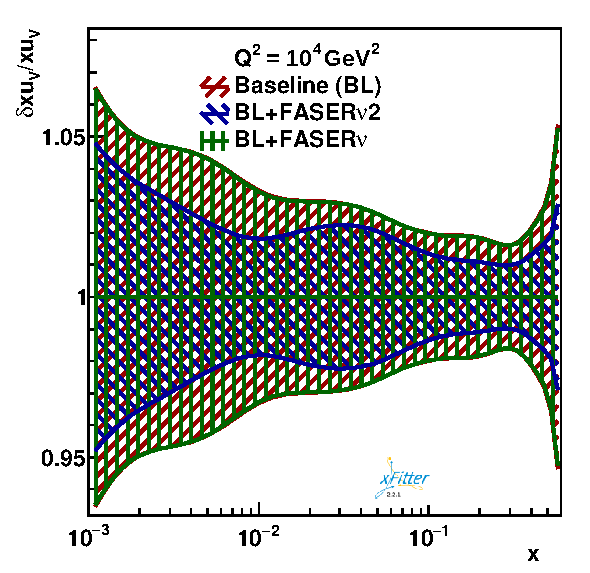
\includegraphics[width=0.32\textwidth]{plots/proton_fasernu2/FASERv2_vs_FASERv/statOnly_FASERv_q2_10000_pdf_uv_ratio.pdf}
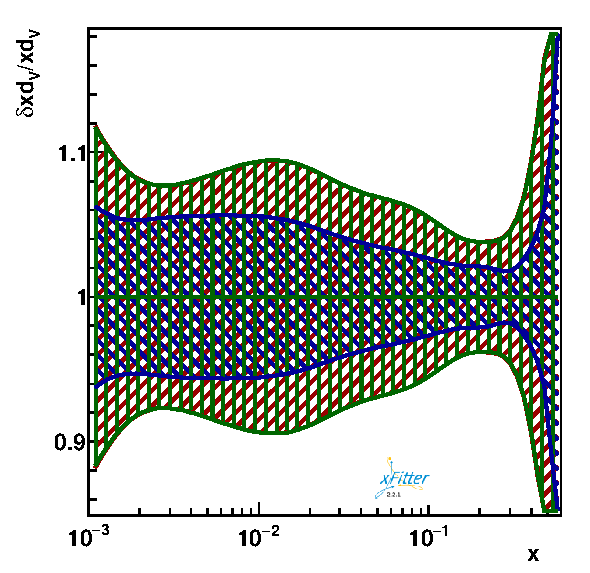
\includegraphics[width=0.32\textwidth]{plots/proton_fasernu2/FASERv2_vs_FASERv/statOnly_FASERv_q2_10000_pdf_dv_ratio.pdf}
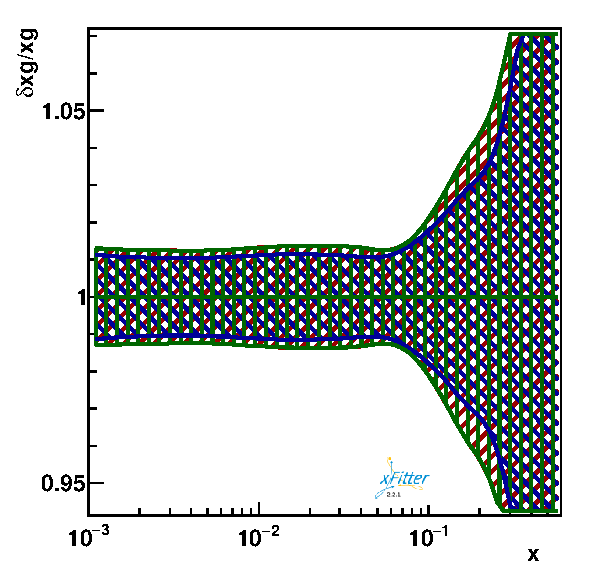
\includegraphics[width=0.32\textwidth]{plots/proton_fasernu2/FASERv2_vs_FASERv/statOnly_FASERv_q2_10000_pdf_g_ratio.pdf}\\
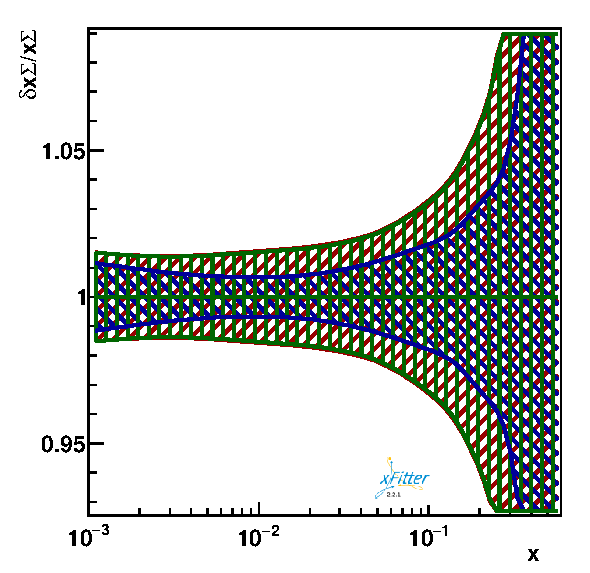
\includegraphics[width=0.32\textwidth]{plots/proton_fasernu2/FASERv2_vs_FASERv/statOnly_FASERv_q2_10000_pdf_Sea_ratio.pdf}
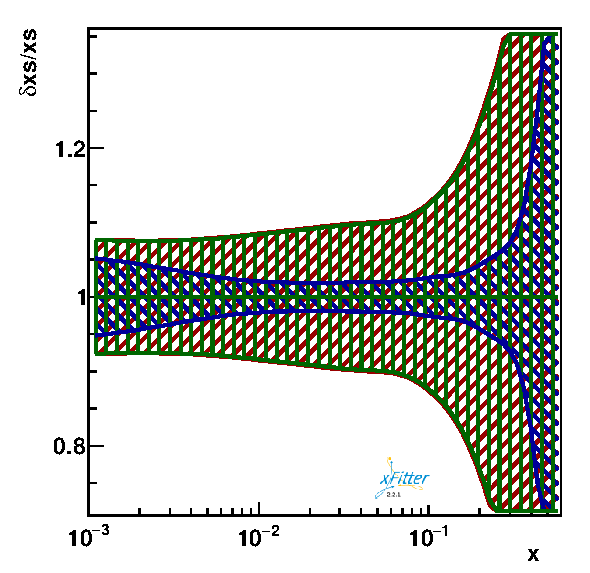
\includegraphics[width=0.32\textwidth]{plots/proton_fasernu2/FASERv2_vs_FASERv/statOnly_FASERv_q2_10000_pdf_s_ratio.pdf}
\caption{Same as  Fig.~\ref{fig:FASERnu2_baseline} (statistical uncertainties only), comparing
  the projected PDF impact of FASER$\nu$2 with that of FASER$\nu$, in the latter
  case assuming the Run III integrated
luminosity of $\mathcal{L}=150$ fb$^{-1}$.
}
\label{fig:FASERnu2_vs_FASERnu}
\end{figure}
%%%%%%%%%%%%%%%%%%%%%%%%%%%%%%%%%%%%%%%%%%%%%%%%%%%%%%%%%%%

It should be emphasized that the lack of PDF sensitivity displayed in Fig.~\ref{fig:FASERnu2_vs_FASERnu}
does not imply that measuring DIS structure functions at FASER$\nu$ will not provide new information.
%
First of all, our procedure assumes perfect compatibility between current data and the projected DIS
neutrino measurements at the LHC, something which remains to be demonstrated experimentally.
%
Second, FASER$\nu$ still covers a region of neutrino energies unexplored by previous experiments, hence providing
a new validation of our QCD calculations and of neutrino interactions at the TeV scale.
%
Third, it would represent a non-trivial proof-of-concept that LHC neutrino differential measurements can be
unfolded to the cross-section level such that they can be used in  theoretical
interpretations, paving the way and demonstrating the feasibility of subsequent neutrino DIS
measurements at the FPF experiments.
